\documentclass[11pt,UTF8]{ctexart}

\usepackage[margin=2cm,a4paper]{geometry}
%\usepackage[left=0.75in,top=0.6in,right=0.75in,bottom=1.0in,a4paper]{geometry}


\setmainfont{Caladea}
%% 也可以選用其它字庫:
% \setCJKmainfont[%
%   ItalicFont=AR PL KaitiM GB,
%   BoldFont=Noto Sans CJK SC,
% ]{Noto Serif CJK SC}
% \setCJKsansfont{Noto Sans CJK SC}
% \renewcommand{\kaishu}{\CJKfontspec{AR PL KaitiM GB}}

% 繁體中文
\setCJKmainfont[Path=fonts/ ]{NotoSansTC-Medium.otf}


\usepackage{minted}
\usepackage[breaklinks]{hyperref}

% Picture
% 導言區的此三行無變化
\usepackage{graphicx}
\usepackage{float} 
\usepackage{subfigure}
% 以下是新增的自定義格式更改
\usepackage[]{caption2} %新增調用的宏包
\renewcommand{\figurename}{Fig.} %重定義編號前綴詞
\renewcommand{\captionlabeldelim}{.~} %重定義分隔符
 %\roman 是羅馬數字編號,\alph是默認的字母編號,\arabic是阿拉伯數字編號,可按需替換下一行的相應位置
\renewcommand{\thesubfigure}{(\roman{subfigure})}%此外,還可設置圖編號顯示格式,加括號或者不加括號
\makeatletter \renewcommand{\@thesubfigure}{\thesubfigure \space}%子圖編號與名稱的間隔設置
\renewcommand{\p@subfigure}{} \makeatother

% Math
\usepackage {mathtools}
\usepackage{amssymb}

% Code
\usepackage{listings}
\usepackage{xcolor}
\lstset{
    % backgroundcolor=\color{red!50!green!50!blue!50},
    % 程式碼塊背景色為淺灰色
    rulesepcolor= \color{gray}, % 程式碼塊邊框顏色
    breaklines=true,  % 程式碼過長則換行
    numbers=left, % 行號在左側顯示
    numberstyle= \small,% 行號字型
    % eywordstyle= \color{red,% 關鍵字顏色
    commentstyle=\color{gray}, % 註釋顏色
    frame=shadowbox % 用方框框住程式碼塊
    }

\usepackage{hyperref}

\title{計算機視覺作業}
\author{干皓丞,2101212850, 信息工程學院}

\begin{document}
\maketitle


\section{題目}

Pytorch 搭建兩層全連接網路

	\begin{lstlisting}[language={python}]
torch.manual_seed(1) # reproducible
x = torch.unsqueeze(torch.linspace(-1, 1, 100), dim=1) 
y = x.pow(2) + 0.2*torch.rand(x.size())
	\end{lstlisting}

\begin{figure}[H]
\centering 
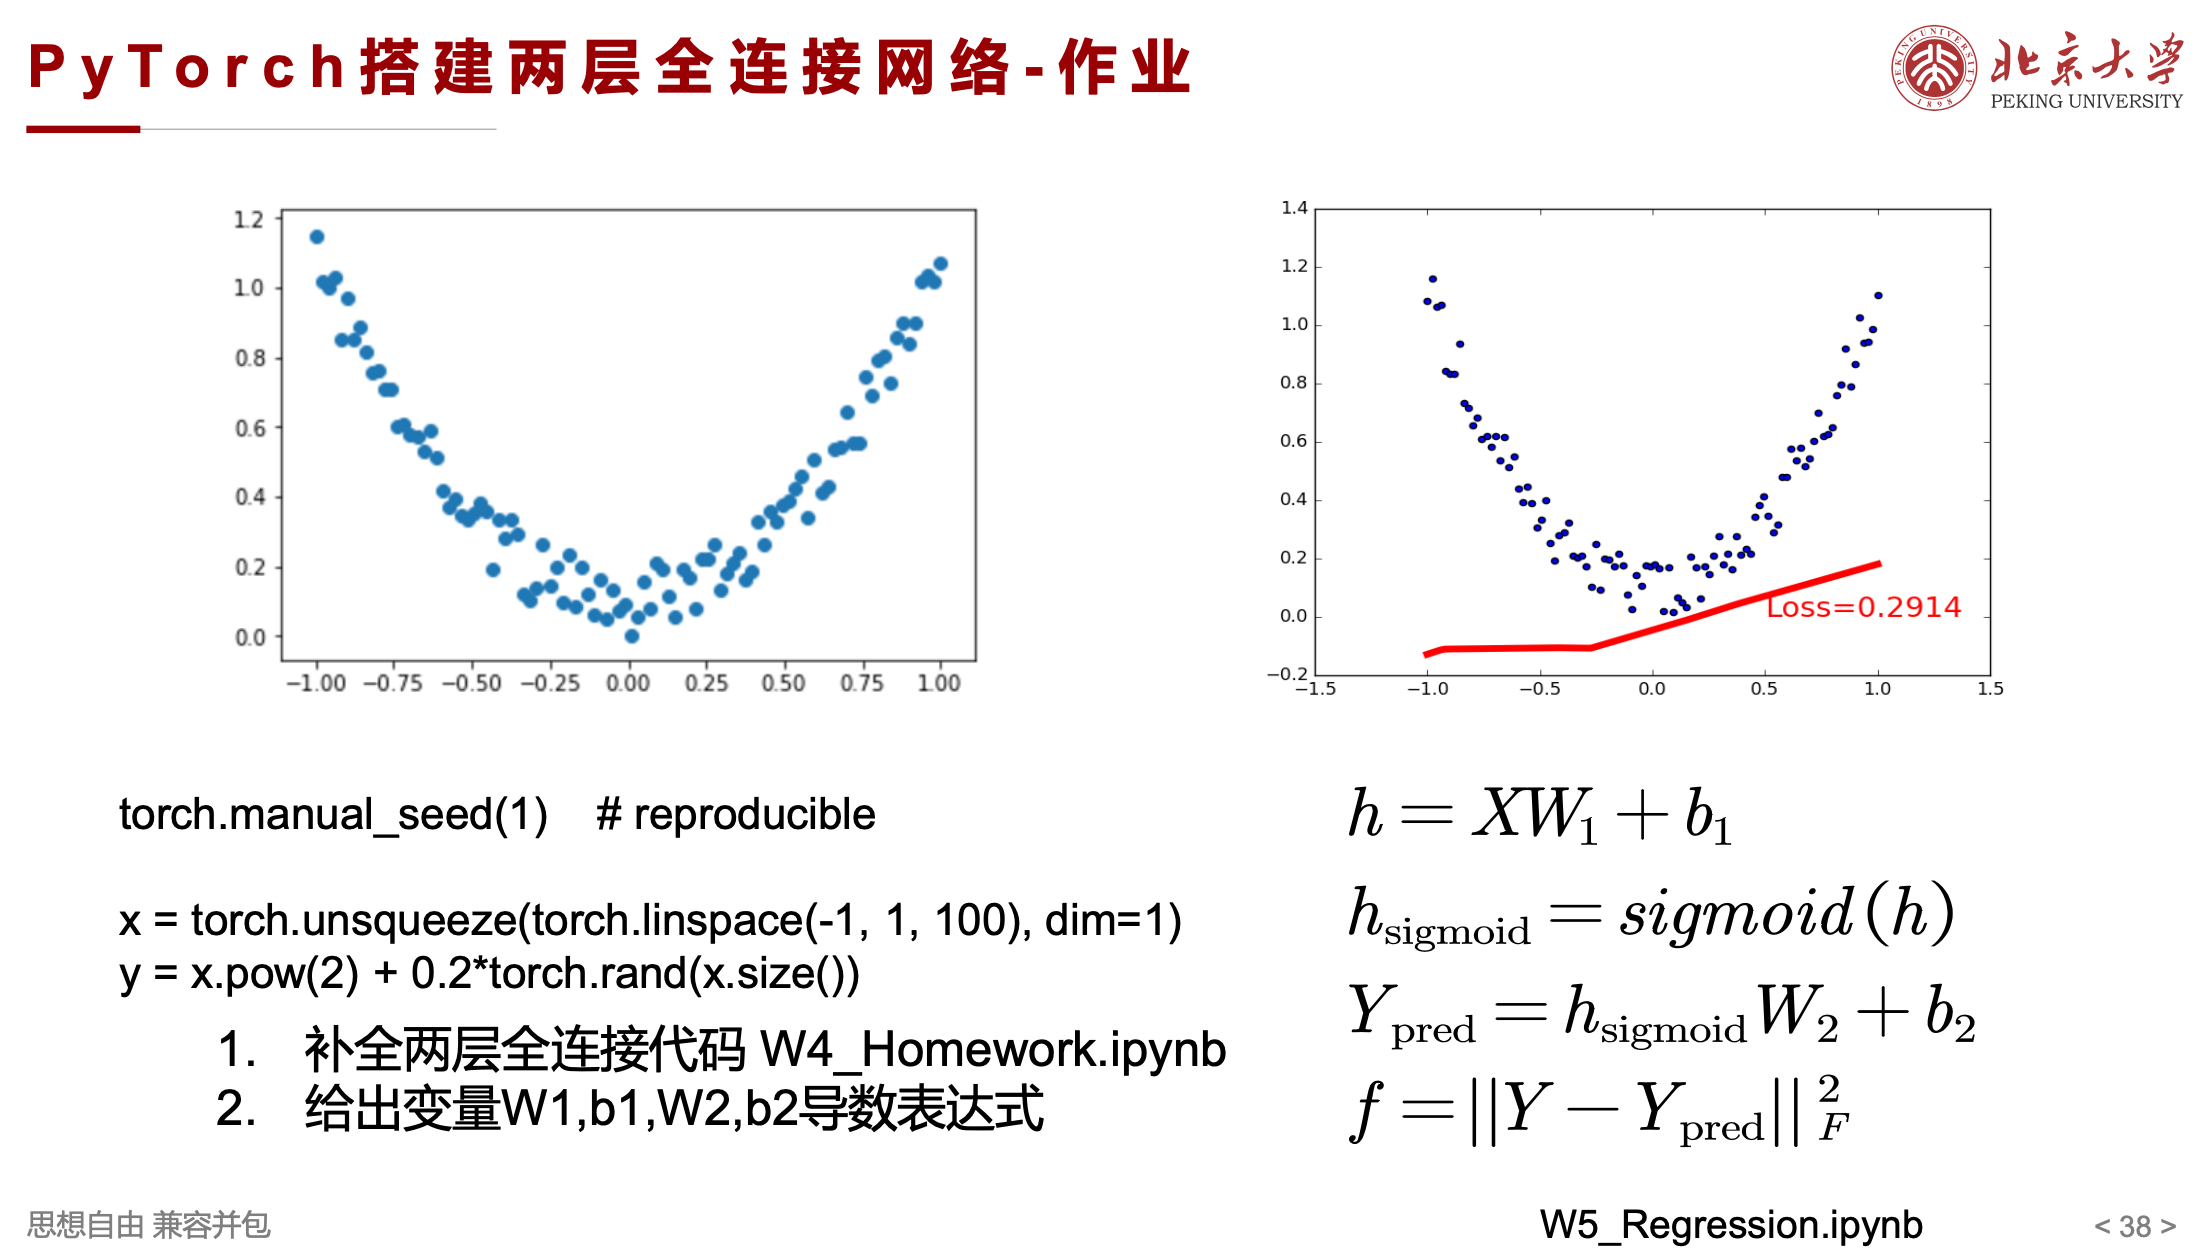
\includegraphics[width=0.9\textwidth]{t1.png} 
\caption{作業目標}
\label{Test}
\end{figure}

1. 補全兩層全連接代碼 W4\_Homework.ipynb

2. 給出變量 W1, b1, W2, b2 導數表達式

目標函數 :

$$f={||\ Y - \ Y_{pred}||}_F^2 \quad \ (1.1)$$

$$ \ h = XW_{1} + b_{1}  \quad \ (1.2);\quad h_{sigmoid} = \ sigmoid(h) \quad \ (1.3);\quad \ Y_{pred} = \ h_{sigmoid}W_{2} + b_{2}  \ (1.4)$$

手推寫出已下表達式,並用 Pytorch 進行實現,在此為了方便表示則省略表達 $Y_{pred}$ 為 $Y_{p}$ ,$h_{sigmoid}$ 則為 $h_{s}$ ,而 $S()$ 即為 Sigmoid 函數,最後數學式 $(1.1)$ 又可以表達如 $(1.5)$。

$$f={||\ Y - \ ( \ S( \ XW_{1} + b_{1}).W_{2} + b_{2} )||}_F^2 \quad \ (1.5)$$

$$ (1)\quad \frac{\partial f}{\partial w1}  \quad (2)\quad \frac{\partial f}{\partial b1} \quad (3)\quad \frac{\partial f}{\partial w2} \quad (4)\quad \frac{\partial f}{\partial b2}$$

\section{數學式定義與程式碼的數學意義說明}

(1) Sigmoid 函數

Sigmoid 函數與函數自身求導的圖形如下所示,紅線為 Sigmoid 函數,藍線為 Sigmoid 函數求導後的函數圖形。

\begin{figure}[H]
\centering  %圖片全局居中
\subfigure[Sigmoid 函數]{
\label{Fig.sub.1}
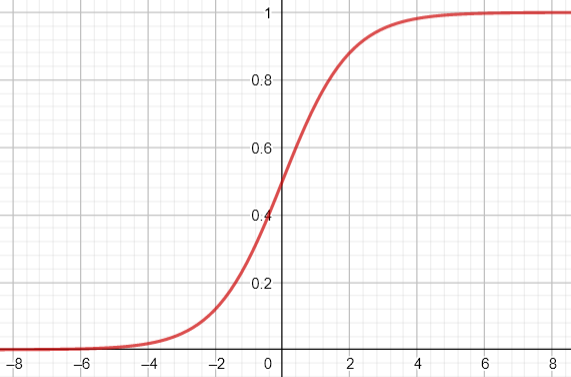
\includegraphics[width=0.45\textwidth]{mp1.png}}
\subfigure[Sigmoid 函數求導與原函數對比]{
\label{Fig.sub.2}
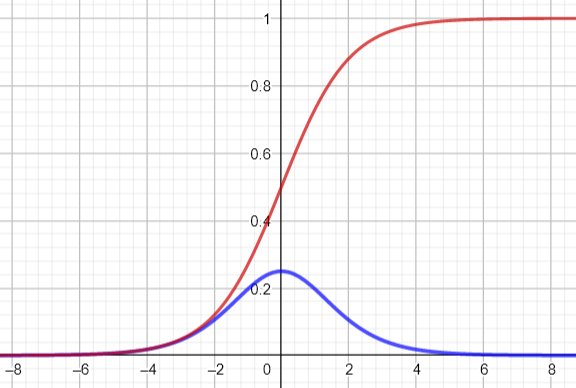
\includegraphics[width=0.45\textwidth]{mp2.png}}
\caption{Sigmoid函數狀態}
\label{Fig.main}
\end{figure}

(2) Sigmoid 定義

Sigmoid 定義如數學式 (2.1) :

$$ \ S(x) = \frac{1}{ \ 1+e^{-x}} =  \frac{e^{x}}{ \ e^{x} + 1} = \ 1 - S(-x) \quad \ (2.1)$$

(3) Sigmoid 求導與推導過程 :

Sigmoid 求導為數學式 (2.2) ,而該函數求導過程則詳見數學式 (2.3) :

$$ \ S'(x) = \ S(x) ( 1 - S(x)) \quad \ (2.2)$$

$$ \frac{d}{dx}\rho(x)\ =\frac{d}{dx}\left[\frac{1}{1+e^{-x}}\right]\ =\ \frac{d}{dx}\ \left[1+e^{-x}\right]^{-1}\ =\ -1\times\left(1+e^{-x}\right)^{-2}\left(-e^{-x}\right)$$

$$=\frac{{-e}^{-x}}{{-(1+e^{-x})}^2}\ =\frac{e^{-x}}{\left(1+e^{-x}\right)^2}\ =\ \frac{1}{1+e^{-x}}\times\frac{e^{-x}}{1+e^{-x}}\ =\ \frac{1}{1+e^{-x}}\times\frac{e^{-x}+(1-1)}{1+e^{-x}}$$

$$=\ \frac{1}{1+e^{-x}}\times\frac{(1+e^{-x})-1}{1+e^{-x}}=\frac{1}{1+e^{-x}}\left[\frac{(1+e^{-x})}{1+e^{-x}}\ -\frac{1}{1+e^{-x}}\right]$$

$$=\frac{1}{1+e^{-x}}\left[1-\frac{1}{1+e^{-x}}\right]=\rho(x)(1-\rho(x))  \quad \ (2.3)$$


(4) 程式碼中的數學意義

	\begin{lstlisting}[language={python}]
import torch
import numpy as np
torch.manual_seed(0)

x = torch.randn(100, 1, requires_grad=True)
y = torch.randn(100, 1, requires_grad=True)
w1 = torch.randn(1, 20, requires_grad=True)
w2 = torch.randn(20, 1, requires_grad=True)
b1 = torch.randn(100, 20, requires_grad=True)
b2 = torch.randn(100, 1, requires_grad=True)
print( "x : ", np.shape(x))
print( "y : ", np.shape(y))
print( "w1 : ", np.shape(w1))
print( "w2 : ", np.shape(w2))
print( "b1 : ", np.shape(b1))
print( "b2 : ", np.shape(b2))
	\end{lstlisting}

\begin{figure}[H]
\centering 
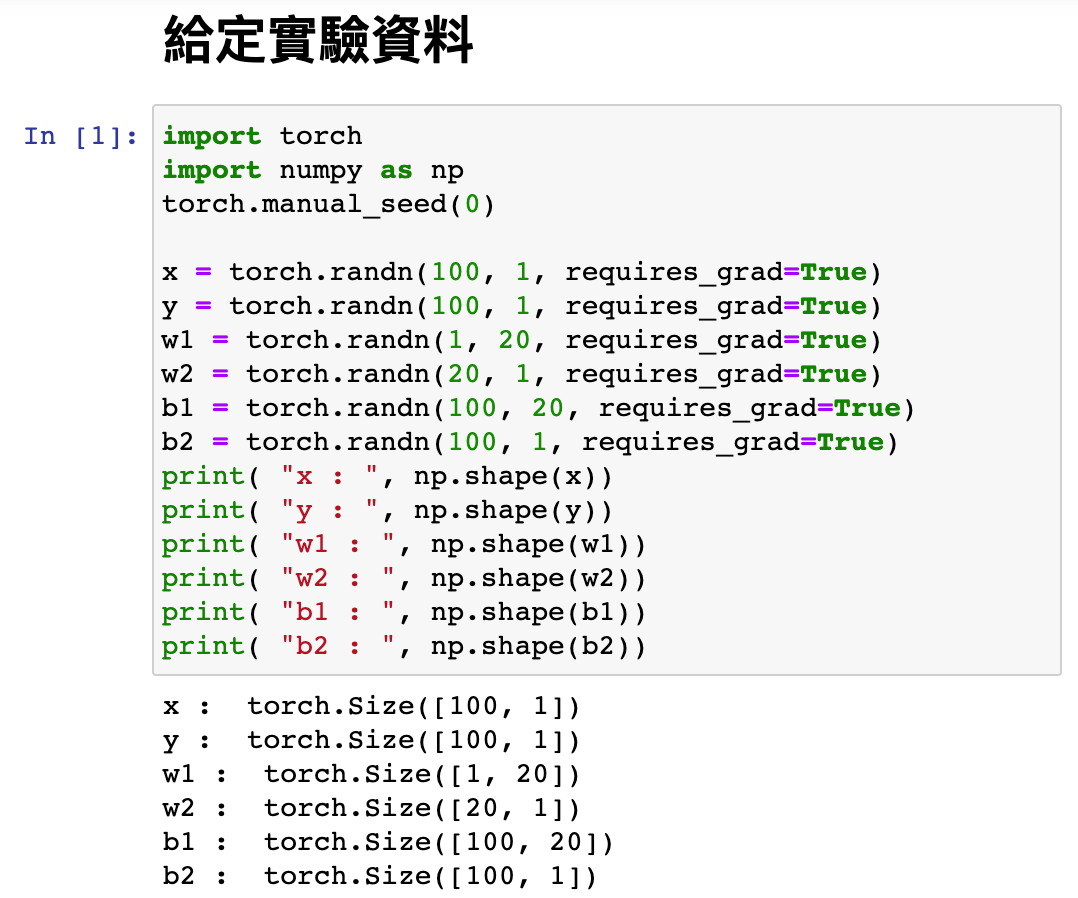
\includegraphics[width=0.7\textwidth]{mcp1.png} 
\caption{Pytorch 矩陣}
\label{Code.2}
\end{figure}

程式碼當中的 x、y、w1、w2、b1、b2 在數學上分別代表了六個矩陣,x、y、b1 皆為 100 X 1 大小的矩陣,w1 矩陣為 1 X 20 大小的矩陣,w2 矩陣為 20 X 1 大小的矩陣,b1 矩陣為 100 X 20 大小的矩陣,而 Pytorch 則會隨機產生矩陣中的值,其數學表達如下。

$$X\ =\ \left[\begin{matrix}\begin{matrix}x_{11}\\x_{21}\\\end{matrix}\\\vdots\\x_{100\ 1}\\\end{matrix}\right]\ ,\ \ Y\ =\ \left[\begin{matrix}\begin{matrix}y_{11}\\y_{21}\\\end{matrix}\\\vdots\\y_{100\ 1}\\\end{matrix}\right]\ ,\ b1\ =\ \left[\begin{matrix}\begin{matrix}{b1}_{11}\\{b1}_{21}\\\end{matrix}\\\vdots\\{b1}_{100\ 1}\\\end{matrix}\right]$$

$$\ \ w1\ =\ \left[\begin{matrix}{w1}_{11}&\ldots&{w1}_{1\ 20}\\\end{matrix}\right]\ ,\ \ w2\ =\ \left[\begin{matrix}{w2}_{11}\\\vdots\\{w2}_{20\ 1}\\\end{matrix}\right],\ \ b1\ =\ \left[\begin{matrix}{b1}_{11}&\ldots&{b1}_{1\ 20}\\\vdots&\ddots&\vdots\\{b1}_{100\ 1}&\ldots&{b1}_{100\ 20}\\\end{matrix}\right]   \quad \ (2.4) $$

% \newpage

\section{數學推導證明}

$$f={||\ Y - \ Y_{pred}||}_F^2 \rightarrow f={||\ Y - \ ( \ S( \ XW_{1} + b_{1}).W_{2} + b_{2} )||}_F^2  \quad \ (3.1)$$

$$ df=\ d(tr({(Y-Y_p)}^T(Y-Y_p)))\ =\ tr(d{(Y-Y_p)}^T(Y-Y_p)+{(Y-Y_p)}^Td(Y-Y_p)) $$

$$tr({2(Y-Y_p)}^Td(Y-Y_p))\ =\ -2tr({(Y-Y_p)}^TdY_p)  \quad \ (3.2)$$

%% \because  \therefore

$$\therefore\quad df=-2tr({(Y-Y_p)}^Tdb_2)\ $$

$$\therefore\quad \frac{\partial f}{\partial b_2}=-2{(Y-Y_p)}^T  \quad \ (3.3)$$

$$df=-2tr({(Y-Y_p)}^T . h_s. dw_2)$$

$$\therefore\quad \frac{\partial f}{\partial w_2}=-2h_s^T.(Y\ -\ Y_p) \quad \ (3.4)$$

$$df=-2tr\left(\left(Y-Y_p\right)^T.{dh}_s. w_2\right)=-2tr\left(\left(\left(Y-Y_p\right).w_2^T\right)^T\left(S(h)\odot(1-S(h))\odot d h\right)\right)$$

$$=-2tr\left(\left(\left(Y-Y_p\right).w_2^T\odot h_s\odot(1-h_s)\right)^T.dh\right)$$

$$\because \ dh = db_{1}$$

$$\therefore\quad \frac{\partial f}{\partial b_1}\ =\ -2(Y-Y_p)w_2^T\odot h_s\odot(1-h_s)  \quad \ (3.5)$$

$$\because \ dh = Xdw_{1}$$

$$\therefore\quad df=-2tr({((Y-Y_p)w_2^T\odot h_s\odot(1-h_s))}^T . x . dw_1)$$

$$\therefore\quad \frac{\partial f}{\partial w_1}\ =\ -2X^T((Y-Y_p)w_2^T\odot h_s\odot(1-h_s)) \quad \ (3.6)$$

% \newpage

\section{Pytorch 程式碼實現}

程式碼可以在 GitHub 專案(kancheng/kan-cs-report-in-2021/CV/pytorch-sigmoid)找到,詳見 sigmoid-math.ipynb 檔案,而範例結果可以從相對應的 PDF 檔案 sigmoid-math.pdf 找到,最後可以發現公式解與程式解兩者結果一致。

(1) Pytorch 實驗資料

下列為 Pytorch 所產生矩陣實驗資料,包含直接求導與手動公式求導,最後會發現兩者結果一致。
\newline

	\begin{lstlisting}[language={python}]
# 給定實驗資料
import torch
import numpy as np
torch.manual_seed(0)

x = torch.randn(100, 1, requires_grad=True)
y = torch.randn(100, 1, requires_grad=True)
w1 = torch.randn(1, 20, requires_grad=True)
w2 = torch.randn(20, 1, requires_grad=True)
b1 = torch.randn(100, 20, requires_grad=True)
b2 = torch.randn(100, 1, requires_grad=True)
print( "x : ", np.shape(x))
print( "y : ", np.shape(y))
print( "w1 : ", np.shape(w1))
print( "w2 : ", np.shape(w2))
print( "b1 : ", np.shape(b1))
print( "b2 : ", np.shape(b2))

# 數學式
import torch.nn as nn
tm = nn.Sigmoid()
hs = tm(x.mm(w1)+b1)
# print(s)
yp = (hs).mm(w2)+b2
f1 = (y - yp).pow(2).sum()
ft = (y - yp).pow(2)
print(f1)
print( "x : ", x.grad)
print( "y : ", y.grad)
print( "w1 : ", w1.grad)
print( "w2 : ", w2.grad)
print( "b1 : ", b1.grad)
print( "b2 : ", b2.grad)
f1.backward()

# 直接求導
print( "x : ", x.grad)
print( "y : ", y.grad)
print( "w1 : ", w1.grad)
print( "w2 : ", w2.grad)
print( "b1 : ", b1.grad)
print( "b2 : ", b2.grad)

# 手動求導
w1_grad = -2 * x.t().mm((y-yp).mm(w2.t()).mul(hs).mul(1-hs))
print( "w1 : ", w1_grad)
w2_grad = -2 * hs.t().mm(y-yp)
print( "w2 : ", w2_grad)
b1_grad = -2 * ((y-yp).mm(w2.t()).mul(hs).mul((1-hs)))
print( "b1 : ", b1_grad)
b2_grad = -2 * (y - yp)
print( "b2 : ", b2_grad)
# 兩者一致
	\end{lstlisting}

\newpage

\section{Pytorch 搭建兩層全連接網路}

程式碼可以在 GitHub 專案(kancheng/kan-cs-report-in-2021/CV/pytorch-sigmoid)找到,詳見 sigmoid-regression.ipynb 檔案,而範例結果可以從相對應的 PDF 檔案 sigmoid-regression.pdf 找到。

	\begin{lstlisting}[language={python}]
%matplotlib inline
import torch
import torch.nn.functional as F
import matplotlib.pyplot as plt
import torch.nn as nn
import numpy as np
torch.manual_seed(1)    # reproducible
# Data
x = torch.unsqueeze(torch.linspace(-1, 1, 100), dim=1)  # x data (tensor), shape=(100, 1)
y = x.pow(2) + 0.2*torch.rand(x.size())
# 繪圖
plt.scatter(x.numpy(), y.numpy())
# 搭建兩層含有 bias 的全連接網路,隱藏層輸出個數為 20 ,激活函數都用 sigmoid()
class Net(torch.nn.Module):
    def __init__(self, n_feature, n_hidden, n_output):
        super(Net, self).__init__()
        self.hidden = torch.nn.Linear(n_feature, n_hidden)
        self.predict = torch.nn.Linear(n_hidden, n_output) # output layer

    def forward(self, x):
        # x = F.relu(self.hidden(x))      # activation function for hidden layer
        # x = self.predict(x) 
        tm = nn.Sigmoid()
        g = tm(self.hidden(x))
        x = self.predict(g)
        return x
net = Net(n_feature=1, n_hidden=20, n_output=1)     # define the network
print(net)  # net architecture
optimizer = torch.optim.SGD(net.parameters(), lr=0.2)
loss_func = torch.nn.MSELoss()  # this is for regression mean squared loss



plt.ion()   # something about plotting

for t in range(201):
    prediction = net(x)     # input x and predict based on x
    loss = loss_func(prediction, y)     # must be (1. nn output, 2. target)

    optimizer.zero_grad()   # clear gradients for next train
    loss.backward()         # backpropagation, compute gradients
    optimizer.step()        # apply gradients

    if t % 20 == 0:
        # plot and show learning process
        plt.cla()
        plt.scatter(x.numpy(), y.numpy())
        plt.plot(x.numpy(), prediction.data.numpy(), 'r-', lw=5)
        plt.text(0.5, 0, 't = %d, Loss=%.4f' % (t, loss.data.numpy()), fontdict={'size': 20, 'color':  'red'})
        plt.pause(0.1)
        plt.show()

plt.ioff()
# plt.show()
	\end{lstlisting}

\clearpage

\end{document}